\secnumbersection{PROPUESTA DE SOLUCIÓN}

% En esta sección (??)

\subsection{Metodología de trabajo}
\label{sec:metod-de-trabajo}

Para nuestro proyecto, buscaremos utilizar una metodología de trabajo orientada a la agilidad. Existen multiples metodologias de este estilo, pero hemos decidido utilizar el ciclo \textit{PDCA}\footnote{PDCA: Del inglés Planear, Hacer, Verificar, Actuar.} (\textit{Plan}, \textit{Do}, \textit{Check}, \textit{Act}) por las siguientes razones.

\begin{itemize}
    \item \textbf{Simple}. Nuestro mayor motivo es que consiste en un proceso simple, directo e intuitivo que podemos adoptar e implementar en nuestro flujo de trabajo, desarrollo e implementación de la solución.
    \item \textbf{Cilcico}. Debido a la naturaleza ciclica e iterativa, \textit{PDCA} nos permite identificar las causas de los posibles errores durante el proceso de desarrollo del proyecto. Además, a medida que se implementan distintas soluciones es posible obtener información y experiencia para comprender el proceso que se busca mejorar.
    \item \textbf{Adaptable}. Esta metodología es una estrategia muy adaptable, aquellas personas que decidan implementarla puede decidir con total libertad que aspectos se deben considerar en cada una de las etapas del ciclo, la unica condición es que las definiciones se deben mantener a lo largo de todo el proceso. Esta adaptabilidad permite que \textit{PDCA} sea altamente esacalable, ya que se puede adaptar a cualquier situación y en organizaciones de cualquier tamaño, incluso, en equipos de una sola persona.
\end{itemize}

\begin{figure}[ht]
    \centering
    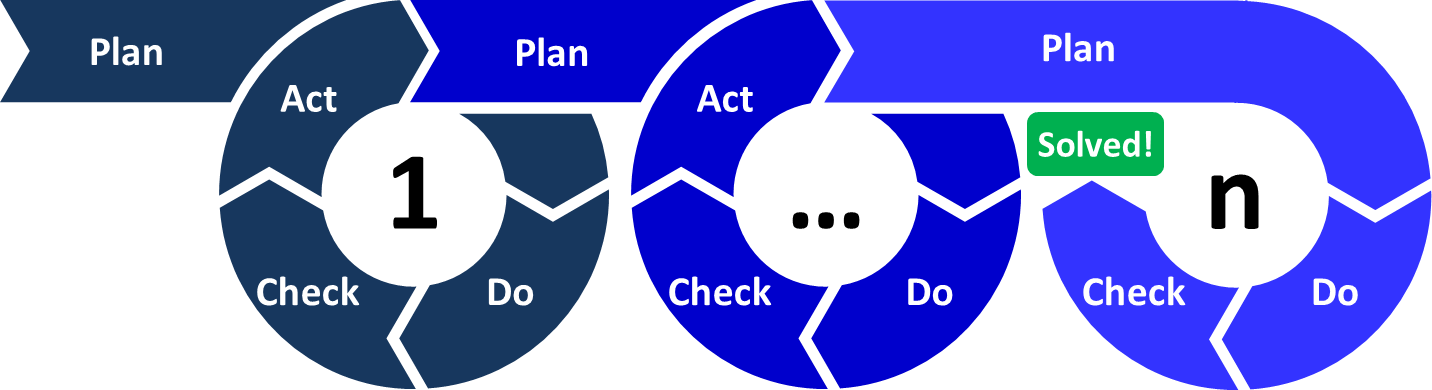
\includegraphics[width=\linewidth]{PDCA-Multi-Loop.png}
    \caption{Ciclos \textit{PDCA}.} Multiples iteraciones del ciclo \textit{PDCA} son realizadas hasta que se logra resolver el problema. Fuente: \textit{PDCA - Wikipedia Commons}.
    \label{fig:pdca-cycle}
\end{figure}

En su esencia \textit{PDCA} es una filosofía para abordar problemas. Primero, identificamos el problema y establecemos nuestros objetivos. Luego, probamos distintos enfoques para alcanzar dichos objetivos, analiszamos nuestros resultados y adaptamos nuestro comportamiento en base a estos. Finalmente, avanzamos la iteración utilizando la solución que ha funcionado.
% TODO: FIXME: REF to https://www.dropbox.com/es/business/resources/pdca

Cada ciclo \textit{PDCA} consiste en las siguientes etapas.

\begin{itemize}
    \item \textbf{Planear}. Debemos comprender nuestro estado actual y el estado deseado. En pocas palabras, esta estapa busca que definamos nuestros objetivos, el cómo alcanzarlos y cómo medir nuestro progreso hacia dichos objetivos.
    \item \textbf{Hacer}. Una vez que hemos definido un plan de acción o una potencial solución para un problema, debemos probarla. Este paso es donde debemos poner a prueba los cambios propuestos en la etapa Planear. Sin embargo, esto se debe considerar como un experimento, no como una solución final. Por lo tanto, todas las pruebas se deben realizar en entornos controlados y a pequeña escala.
    \item \textbf{Verificar}. Luego de completar nuestras pruebas, debemos comprobar que los cambios o soluciones propuestas tienen el efecto deseado. En esta etapa se debe analizar la información recopilada durante la etapa Hacer y comparar lo obtenido con los objetivos y metas originales. En resumen, debemos evaluar nuestro nivel de éxito y qué cosas vamos a conservar para el siguiente paso del ciclo.
    \item \textbf{Actuar}. Al llegar a esta etapa, ya hemos logrado identificar una solución o propuesta de cambio para implementar en nuestro problema o proceso. Se deben aplicar estos cambios en la escala que sea necesaria por el proceso y con esto se definen las bases para una nueva iteración.
\end{itemize}

\subsection{Plan de trabajo}
\label{sec:plan-de-trabajo}

Como hemos mencionado anteriormente, vamos a utilizar cilcos \textit{PDCA} para encontrar la solución a nuestro problema, estos ciclos, son definidos conforme avanzamos en las iteraciones y debido a que se encuentra en el marco de las metodologias agiles, seria irresponsable definir con antelación los objetivos de cada ciclo. Sin embargo, podemos definir determinados hitos que buscamos lograr durante todo este proceso, los cuales, detallamos a continuación.

\begin{enumerate}
    \item Entender la arquitectura inicial de la solución existente (\textit{SPARQLforHumans}).
    \item Diseñar y definir una arquitectura acorde a nuestras restricciones.
    \item Reducir significativamente el tiempo necesario para ejecutar la solución.
    \item Diseñar y definir una arquitectura que permita la actualización en tiempo real de los datos utilizados por nuestra solución.
    \item Actualizar los datos de nuestra solución en tiempo real.
    \item Validar la solución a través de pruebas unitarias automatizadas.
\end{enumerate}

Estos hitos, nos permitiran guiar las iteraciones de nuestro proceso \textit{PDCA} y así no perder el rumbo durante la implementación.

Con las definiciones realizadas en las secciones \ref{sec:metod-de-trabajo} y \ref{sec:plan-de-trabajo} tenemos los necesario para comenzar nuestras iteraciones.

\subsection{Primera iteración: Analisis inicial de la solución existente}

\subsubsection*{Planificación}

Para nuestra primera iteración, nuestro objetivo es entender el proceso y los componentes de la aplicación \textit{SPARQLforHumans}, para esto, revisaremos el código fuente disponible de forma publica \cite{parra2020autocompletion}.

\subsubsection*{Implementación}

Comenzaremos con entender el proceso. Al revisar el código fuente de la aplicación, logramos identificar las siguientes etapas.

\begin{enumerate}
    \item Inicio de la aplicación.
    \begin{enumerate}
        \item Lectura de un fichero en el formato de compresión \textit{gzip} \cite{rfc1952} desde \textit{Wikidata}.
        \item Filtro y validación de lineas en formato \textit{N-Triples}.
        \item Creación de objetos \textit{Triple} en base a lineas validas.
        \item Generación de propiedades inversas para determinadas entidades.
        \item Concatenación de lineas validas y nuevas propiedades a nuevo fichero \textit{gzip}.
        \item Ordenar lineas de nuevo fichero en función de la entidad \textit{RDF} observada en cada linea.
    \end{enumerate}
    \item Indexación de entidades.
    \begin{enumerate}
        \item Lectura de nuevo fichero \textit{gzip} generado anteriormente.
        \item Creación de objetos \textit{Triple}.
        \item Generación de documentos en indice \textit{Lucene} en base a propiedades de cada entidad.
    \end{enumerate}
    \item Obtención del valor \textit{PageRank} para entidades.
    \item Indexación de propiedades.
    \begin{enumerate}
        \item Lectura de documentos disponibles en indice \textit{Lucene} para entidades.
        \item Calculo de frecuencias para las propiedades existentes en los distintos documentos.
        \item Generación de documentos en nuevo indice \textit{Lucene} en función de la frecuencia de cada propiedad identificada.
    \end{enumerate}
    \item Sistema en vivo.
    \begin{enumerate}
        \item Ejecución de prueba estadistica y de rendimiento.
        \item Inicio de servidor Web.
    \end{enumerate}
\end{enumerate}

Las interacciones entre cada etapa se puede observar en el diagrama de procesos presentado en la figura \ref{fig:sfh-bpmn} y los componentes identificados se pueden observar en la figura \ref{fig:sfh-componentes}. Además, presentamos la arquitectura actual del sistema en la figura TODO.

\begin{figure}[ht]
    \centering
    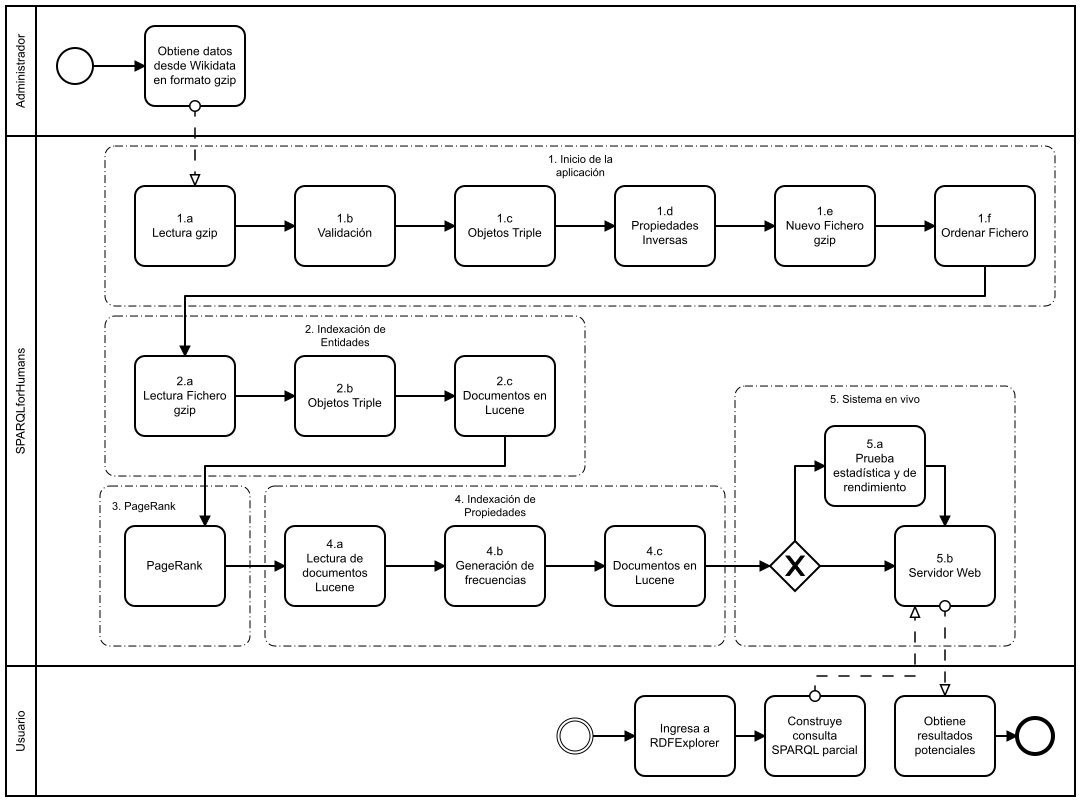
\includegraphics[width=\linewidth]{sparqforhumans_process_bpmn}
    \caption{Proceso de arranque de la aplicación \textit{SPARQLforHumans}.}Fuente: Elaboración Propia.
    \label{fig:sfh-bpmn}
\end{figure}

\begin{figure}
    \centering
    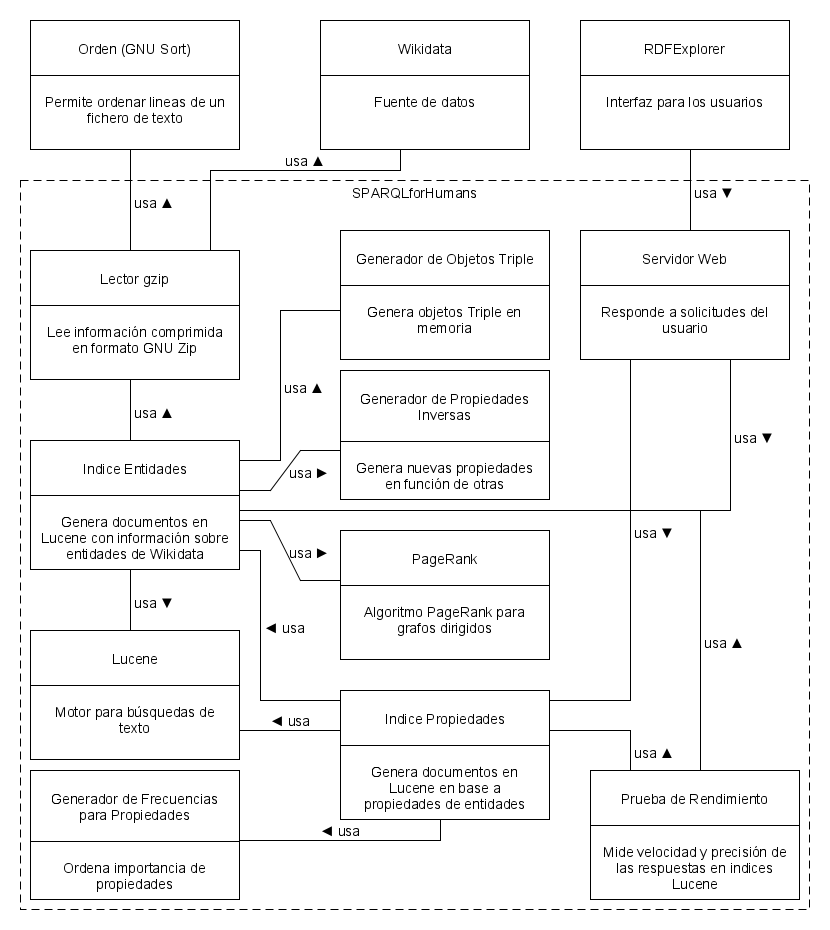
\includegraphics[width=\linewidth]{sfh_comm}
    \caption{Diagrama de componentes para la aplicación \textit{SPARQLforHumans}.}Fuente: Elaboración Propia.
    \label{fig:sfh-componentes}
\end{figure}

\subsubsection*{Resultados}

Gracias al levantamiento de proceso y componentes realizado, podemos ver de forma más clara cómo interactuan cada uno de los distintos modulos de la aplicación existente. Esto nos permite entender su funcionamiento interno, de forma tal, que podemos comenzar a optimizar cada uno de los componentes identificados por separado, acercandonos a nuestro objetivo final.

\subsection{Segunda iteración: Mejoras al rendimiento general}

\subsubsection*{Planificación}

Nuestra segunda iteración consiste en diseñar e implementar el conjunto de mejoras iniciales al rendimiento de la solución. Para lograr esto, comenzaremos con un nuevo diseño y una nueva implementación desde cero, en el lenguaje de programación basado en la \textit{JVM},\footnote{Del inglés. \textit{Java Virtual Machine}.} \textit{Kotlin}\footnote{\textit{The Kotlin Programming Language.} \href{https://kotlinlang.org/}{https://kotlinlang.org/}}. Nuestra implementación se encuentra disponible en un repositorio publico dentro de la plataforma GitHub\footnote{\href{https://github.com/capgadsx/SPARQLforHumans}{https://github.com/capgadsx/SPARQLforHumans}}.

Para esta iteración, definiremos nuestro progreso en función de la cantidad de tiempo reducido en el proceso de arranque de nuestra aplicación. Es decir, desde el punto \texttt{(1.a)} hasta el punto \texttt{(5.b)} de nuestro proceso. Cómo objetivo, hemos definido reducir en al menos un $50\%$ este tiempo de $109$ horas.

\subsubsection*{Implementación}

Comenzaremos aclarando nuestra decisión de utilizar \textit{Kotlin} y la \textit{JVM} para la implementación de nuestra solución. Algo importante a notar es que \textit{SPARQLforHumans} fue escrito utilizando el \textit{.NET Framework} del lenguaje \textit{C\#}, sin embargo, el proyecto \textit{Apache Lucene}\footnote{\href{https://lucene.apache.org/}{https://lucene.apache.org/}} utilizado como el corazón de la solución esta desarrollado en el lenguaje \textit{Java}, por lo que se utiliza una biblioteca de compatibilidad llamada \textit{Lucene.NET}\footnote{\href{https://lucenenet.apache.org/}{https://lucenenet.apache.org/}}. Para nuestra solución, buscamos utilizar el proyecto original, \textit{Apache Lucene}, por lo que deberiamos utilizar \textit{Java}.

Pero no utilizaremos \textit{Java}, como hemos mencionado anteriormente, vamos a utilizar \textit{Kotlin}. \textit{Kotlin} es un lenguaje de programación moderno, maduro y versátil, el cual busca facilitar el desarrollo de aplicaciones. Es consiso, seguro y completamente interoperable con \textit{Java} y otros lenguajes que se ejecutan en la \textit{Java Virtual Machine}. Por lo tanto, podemos utilizar sin problemas todas las funcionalidades de \textit{Apache Lucene} a través de un lenguaje más moderno como \textit{Kotlin}.

Lo siguiente es comentar sobre la implementación realizada. Nuestra solución de referencia corresponde a un sistema monolítico y para nuestras primeras mejoras vamos a seguir este modelo de arquitectura. En resumen, hemos realizado lo siguiente.

\begin{itemize}
    \item Hemos eliminado el modulo de orden. En vez de ordenar nuestros resultados al final del subproceso \texttt{(1)}, vamos a utilizar una estructura de datos llamada \textit{TreeMap},\footnote{\textit{TreeMap}: Un diccionario llave-valor, el cual, al ser recorrido de forma lineal entrega sus llaves de forma ordenada. \href{https://docs.oracle.com/javase/8/docs/api/java/util/TreeMap.html}{https://docs.oracle.com/javase/8/docs/api/java/util/TreeMap.html}} la cual nos permite mantener ordenados las propiedades inversas y objetos \textit{Triple} generados en base al identificador de la entidad que actualmente estamos procesando, cómo por ejemplo $Q88618255$, sin la necesidad de utilizar una herramienta externa como \textit{gzip} o \textit{sort}. Este cambio nos permite eliminar las etapas \texttt{(1.e)} y \texttt{(1.f)} de nuestra nueva solución.
    \item Hemos modernizado el componente que interactua con \textit{Lucene}, utilizando la ultima versión disponible para el formato de indices y la clase \textit{MMapDirectory}\footnote{\href{https://lucene.apache.org/core/8\_9\_0/core/org/apache/lucene/store/MMapDirectory.html}{https://lucene.apache.org/core/8\_9\_0/core/org/apache/lucene/store/MMapDirectory.html}} para interactuar con estos, la cual, corresponde a una interfaz de alto rendimiento que logra aprovechar el \textit{cache} del sistema operativo donde se ejecuta.
    \item Hemos utilizado la biblioteca \textit{Apache Jena}\footnote{\href{https://jena.apache.org/}{https://jena.apache.org/}} para generar objetos \textit{Triple}, esto nos permite generar nuevas propiedades y \textit{Triples} de forma sencilla.
    \item El resto de componentes, han sido implementados en \textit{Kotlin} sin cambios significativos con la implementación de referencia.
\end{itemize}

Para realizar nuestras pruebas y obtener resultados, hemos definido los siguientes ambientes.

\begin{enumerate}
    \item Ambiente de desarrollo.
    \begin{itemize}
        \item Conjunto de datos: \textit{200MB} de datos \textit{N-Triple} comprimidos en formato \textit{gzip}.
        \item Recursos.
        \begin{itemize}
            \item \textit{CPU}. Intel(R) Core(TM) i5-7200U CPU @ 2.50GHz, 4 nucleos.
            \item \textit{RAM}. \textit{7GB}.
            \item Almacenamiento. Samsung SSD 960 EVO 250GB. Interfaz NVME.
        \end{itemize}
    \end{itemize}
    \item Ambiente de pruebas.
    \begin{itemize}
        \item Conjunto de datos: \textit{1GB} de datos \textit{N-Triple} comprimidos en formato \textit{gzip}.
        \item Recursos.
        \begin{itemize}
            \item \textit{CPU}. Intel(R) Core(TM) i5-3470 CPU @ 3.20GHz, 4 nucleos.
            \item \textit{RAM}. \textit{10GB}.
            \item Almacenamiento. Seagate 320GB 7.2K SATA 3.5 HDD.
        \end{itemize}
    \end{itemize}
    \item Ambiente de producción.
    \begin{itemize}
        \item Conjunto de datos: \textit{45GB} de datos \textit{N-Triple} comprimidos en formato \textit{gzip}.
        \item Recursos, (Amazon AWS EC2 Instance - t3.2xlarge).
        \begin{itemize}
            \item \textit{CPU}. Intel(R) Xeon(R) Platinum 8259CL CPU @ 2.50GHz, 8 nucleos.
            \item \textit{RAM}. \textit{32GB}.
            \item Almacenamiento. Amazon AWS EBS, General Purpose SSD (gp2) 200GB. Interfaz NVME.
        \end{itemize}
    \end{itemize}
\end{enumerate}

Al realizar pruebas en pequeña escala, los resultados son alentadores, pero hemos notado un problema, no estamos utilizando de forma eficiente los recursos disponibles de nuestro entorno de ejecución, especialmente nuestra memoria \textit{RAM}.

En la figura \ref{fig:i2-prof-htop}, podemos notar que solo estamos utilizando un $25\%$ de nuestra \textit{CPU} disponible y una gran parte de la memoria \textit{RAM} del sistema, durante toda la ejecución de nuestra aplicación.

\begin{figure}[ht]
    \centering
    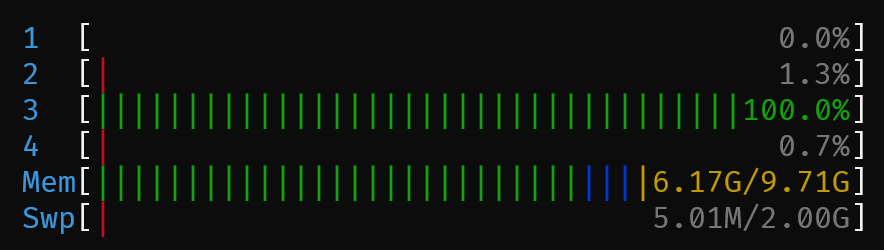
\includegraphics[width=\linewidth]{profiler-memoria-cpu1.png}
    \caption{Utilización de recursos, \textit{CPU} y \textit{RAM} en ambiente de desarrollo.}Fuente: Elaboración Propia.
    \label{fig:i2-prof-htop}
\end{figure}

A pesar de esto, hemos decidido ejecutar el proceso en el ambiente de producción, para así obtener una metrica sobre el tiempo de arranque de nuestra solución. Lamentablemente, solo logramos obtener un error del tipo \textit{java.lang.OutOfMemoryError} despues de unas cuantas horas de ejecución.

La excepción \textit{java.lang.OutOfMemoryError} es un indicador común de una fuga de memoria. Normalmente, este error se genera cuando no hay espacio suficiente para asignar un objeto en el \textit{stack}\footnote{TODO.} de la \textit{JVM}. En este caso, el recolector de basura no puede hacer espacio disponible para acomodar un nuevo objeto, y el \textit{heap}\footnote{TODO.} no puede expandirse más. También, este error puede ser lanzado cuando no hay suficiente memoria nativa para soportar la carga de una nueva clase en la \textit{JVM}. En un casos extremadamente raros, un error del tipo \textit{java.lang.OutOfMemoryError} puede ser lanzado cuando se está gastando una cantidad excesiva de tiempo en la recolección de basura y poca memoria está siendo liberada.

En nuestro caso, creemos que este error se debe a que no es posible acomodar nuevos objetos en nuestra memoria. Además, buscamos saber donde estamos utilizando nuestra \textit{CPU}, con el objetivo de implementar potenciales optimizaciones. Para lograr esto, debemos responder las siguientes preguntas.

\begin{enumerate}
    \item ¿Donde se esta utilizando la \textit{CPU}?
    \item ¿Donde se estan creando los objetos que utilizan nuestra memoria \textit{RAM}?
    \item ¿Que objetos son los que se encuentan en nuestra memoria \textit{RAM}?
\end{enumerate}

Esta clase de dudas pueden ser resueltas utilizando un tipo especifico de herramientas. profilers.

Para responder a nuestra primera incognita, podemos utilizar una herramienta llamada \textit{Java Flight Recorder}\footnote{TODO}, la cual, nos permite medir y grabar lo que se esta ejecutando en la \textit{JVM}. Con esta herramienta podemos generar la figura \ref{fig:i2-prof-jfr}, donde se puede observar una lista de métodos junto con el porcentaje del tiempo que fueron ejecutados en referencia al total del tiempo de ejecución de nuestro programa.

\begin{figure}[ht]
    \centering
    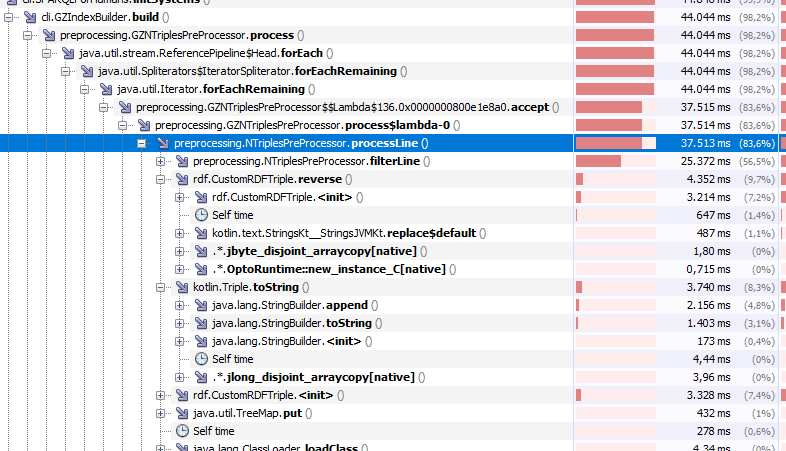
\includegraphics[width=\linewidth]{profiler-string-time.png}
    \caption{Reporte generado por \textit{JFR}.}Fuente: Elaboración Propia.
    \label{fig:i2-prof-jfr}
\end{figure}

Podemos notar, que el $98.2\%$ del tiempo, la \textit{CPU} esta siendo utilizado por el método \texttt{process} de la clase \texttt{GZNTriplesPreProcessor}, el cual, utiliza a \texttt{processLine} y \texttt{filterLine}, ambos de la clase \texttt{NTriplesPreProcessor} y a \texttt{reverse} de la clase \texttt{CustomRDFTriple}. Estos métodos, son los encargados de leer, validar y procesar cada linea del fichero en formato \textit{gzip} utilizado como entrada de nuestra aplicación. Esto significa que no hemos logrado avanzar de las etapas \texttt{(1.b), (1.c)} y \texttt{(1.d)} en nuestra solución.

\begin{figure}[ht]
    \centering
    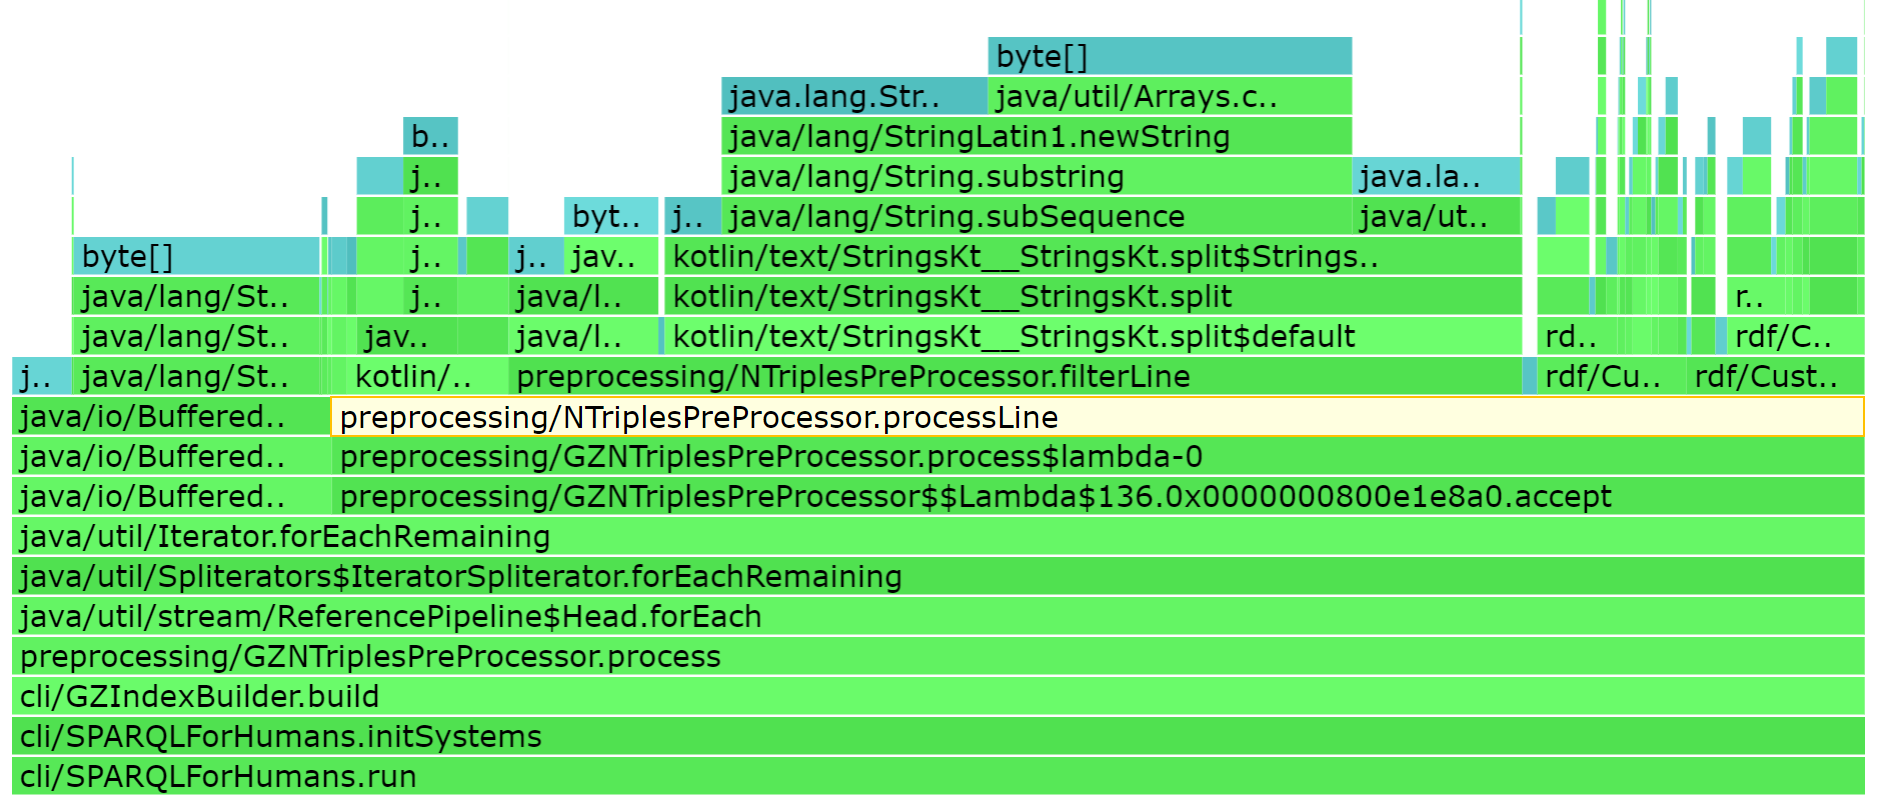
\includegraphics[width=\linewidth]{profiler-mem-flame.png}
    \caption{Reporte generado por \textit{Async-Profiler}.}Fuente: Elaboración Propia.
    \label{fig:i2-prof-mem}
\end{figure}

Para las segunda y tercera preguntas, podemos utilizar el grafico de la figura \ref{fig:i2-prof-mem}, generado por la herramienta \textit{Async-Profiler}\footnote{TODO.}. Esta figura, corresponde a una representación de aquellas funciones que han generado los objetos que se encuentran en la memoria de la \textit{JVM} en un momento determinado. Podemos notar algunos puntos importantes en esta representación.

\begin{itemize}
    \item La mayor parte de los objetos han sido generados desde \texttt{processLine}.
    \item La mayor parte de los objetos corresponden a \texttt{Strings} o \texttt{byte[]}.
    \item Los objetos generados esta fuertemente relacionados a operaciones de separación, subsequencias y concatenación de cadenas de texto (\texttt{String}).
\end{itemize}

Ahora, con el proceso, el código fuente de nuestra implementación y esta nueva información podemos concluir que la causa de nuestro error \textit{java.lang.OutOfMemoryError} es la existencia de multiples objetos del tipo \texttt{String} que no han sido liberados de la memoria durante la ejecución de nuestra solución. Esto se puede observar en más detalle a través de la figura \ref{fig:i2-prof-mem-allocs}.

\begin{figure}[ht]
    \centering
    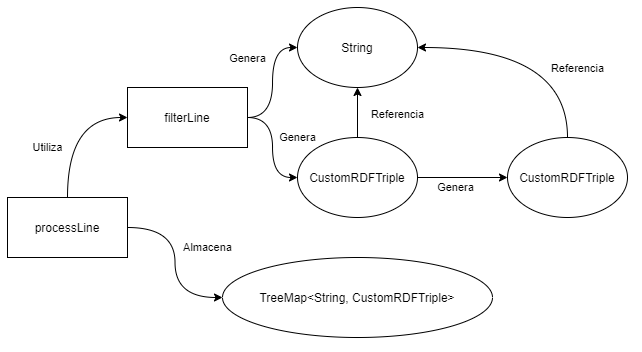
\includegraphics[width=\linewidth]{mem-allocs-jvm.png}
    \caption{Generación de objetos \texttt{CustomRDFTriple}.}Fuente: Elaboración Propia.
    \label{fig:i2-prof-mem-allocs}
\end{figure}

En la figura se puede observar que la función \texttt{processLine} utiliza a \texttt{filterLine} para generar objetos del tipo \texttt{CustomRDFTriple}, el cual a su vez, puede generar otro objeto \texttt{CustomRDFTriple} en función de sus propiedades inversas. Estos, utilizan objetos \texttt{String} para interactuar con la biblioteca \textit{Apache Jena} y obtener determinada información sobre los \textit{Triples} que representan. Aquellos \texttt{Strings} son almacenados como propiedades de los \texttt{CustomRDFTriples}. Finalmente, ambos \texttt{CustomRDFTriples} son almacenados de forma ordenada en una instancia \texttt{TreeMap}.

Toda esta nueva información sobre las necesidades funcionales de la aplicación nos hacen cuestionar la decisión de utilizar \textit{Kotlin} y la \textit{JVM} para procesar grandes cantidades de texto.

\subsubsection*{Resultados}

No hemos logrado nuestro objetivo en esta iteración, debido a que no logramos ejecutar completamente nuestra solución. Sin embargo, no todo es malas noticias, hemos obtenido información valiosa para continuar en el desarrollo de la solución. En resumidas cuentas, lo siguiente.

\begin{itemize}
    \item Debemos realizar una implementación que utilize una menor cantidad de memoria \textit{RAM} del sistema.
    \item Debemos paralelizar nuestra solución, de esta forma, utilizaremos de forma más eficiente nuestra \textit{CPU} y lograremos acercarnos aún más a nuestro objetivo.
    \item Existe una optimización importante en la etapa \texttt{(3 - PageRank)}, puesto que, se está utilizando una implementación iterativa del algoritmo. Funciona en pequeña escala, pero al utilizar una cantidad real de $90$ millones de nodos, definitivamente nos va a tomar tiempo procesar todo.
\end{itemize}

Con toda esta nueva información y nuevas necesidades, estamos listos para volver a intentar alcanzar nuestro objetivo de reducir en un $50\%$ nuestro tiempo de arranque en una nueva iteración.

\subsection{Tercera iteración: Desacoplamiento de componentes, \textit{Message Brokers} y codificación binaria}

\subsubsection*{Planificación}

A

\subsubsection*{Implementación}

A

\subsubsection*{Resultados}

A

\subsection{Cuarta iteración: Paralelización de etapas}

\subsubsection*{Planificación}

A

\subsubsection*{Implementación}

A

\subsubsection*{Resultados}

A

\subsection{Quinta iteración: Actualización de resultados en tiempo real}

\subsubsection*{Planificación}

A

\subsubsection*{Implementación}

A

\subsubsection*{Resultados}

A

\subsection{Sexta iteración: Optimizaciones de transporte}

\subsubsection*{Planificación}

A

\subsubsection*{Implementación}

A

\subsubsection*{Resultados}

A

\subsection{Septima iteración: Implementación de pruebas}

\subsubsection*{Planificación}

A

\subsubsection*{Implementación}

A

\subsubsection*{Resultados}

A

